%! TEX root = ../main.tex
In this section, we study intergenerational income mobility in Chile with informality. In particular, we replicate the estimates of \citet{nunez2010mobility}: first-stage earnings equations (Table~A) and two-sample two-stage least squares (TSTSLS) elasticities (Table~1) using CASEN 1987, 1990 and 2006.

To account for the absence of linked father-son income records, we follow the TSTSLS methodology: historic earnings equations predict paternal income from retrospective characteristics reported by sons, and the predicted income enters a second-stage regression with a Murphy-Topel correction \citep{murphy1985estimation}.

Finally, we extend the analysis beyond the original paper in two directions: (i) rank-rank regressions by pension-contribution status, and (ii) multiple imputation of paternal income and affiliation under alternative residual-correlation scenarios \citep{vanbuuren2018flexible,kim2016statistical}.

\subsection{Historic Earnings Equations}\label{sec:first-stage}
For each historic year $t \in \{1987, 1990\}$ we estimate by OLS the log of monthly labor income. $E$ contains four indicators of completed schooling level: primary, secondary, technical and university; the omitted category is no schooling or incomplete primary. Age is denoted by $a$:
\begin{equation}
    L_{jt} = \alpha_t + E_{jt}^{\prime}\gamma_t + \delta_{1t}a_{jt} + \delta_{2t}a_{jt}^2 + u_{jt}, \quad L = \log y.
    \label{eq:earn-a}
\end{equation}
The extended specification adds occupation indicators $O$ for employer, self-employed and domestic service; employees and laborers are the occupational reference:
\begin{equation}
    L_{jt} = \alpha_t + E_{jt}^{\prime}\gamma_t + O_{jt}^{\prime}\pi_t + \delta_{1t}a_{jt} + \delta_{2t}a_{jt}^2 + u_{jt}.
    \label{eq:earn-b}
\end{equation}
The first-stage samples are males aged 15--55, employed ($o21=1$), with positive labor income: $N=18{,}769$ (1987) and $N=20{,}387$ (1990); with occupation the samples are $18{,}441$ and $20{,}354$ respectively.\footnote{See \texttt{source/mobility.py} (\texttt{recode\_1987}, \texttt{recode\_1990}, \texttt{build\_sample}) and \texttt{notebooks/07\_nunez\_miranda.ipynb}, Sec.~1. In 1987 income sums \textit{ysefaj}, \textit{yganaj} and \textit{yespaj}; in 1990 and 2006 it is \textit{ytrabaj}.} Table~\ref{tab:mob-a} reports the replication of Table~A: schooling coefficients are positive and increasing, and the estimates match the reference implementation to four decimals.\footnote{Reference values from the author's replication files; standard errors are HC1.}

\begin{table}[H]
    \centering
    \caption{First-stage earnings equations (Table~A)}\label{tab:mob-a}
    \begin{tabular}{lcc}
        \toprule
        & CASEN 1987 & CASEN 1990 \\
        \midrule
        Complete primary & 0.2538 [0.0124] & 0.2132 [0.0117] \\
        Complete secondary & 0.7564 [0.0141] & 0.6315 [0.0136] \\
        Complete technical & 1.0638 [0.0725] & 0.9426 [0.0404] \\
        Complete university & 1.7927 [0.0271] & 1.4808 [0.0284] \\
        Age & 0.0777 [0.0037] & 0.0657 [0.0035] \\
        Age$^2$ & -0.0008 [0.0001] & -0.0006 [0.0000] \\
        Constant & 8.1609 [0.0612] & 9.1366 [0.0578] \\
        Observations & 18,769 & 20,387 \\
        Adj.\ R-squared & 0.35 & 0.29 \\
        \bottomrule
    \end{tabular}
    \vspace{0.2em}
    \flushleft\footnotesize{\textit{Note:} Dependent variable: log earnings. HC1 robust standard errors in brackets.}
\end{table}

\subsection{TSTSLS Elasticities}\label{sec:tsts}
In CASEN 2006, retrospective questions record paternal schooling (\textit{t14a}) and occupation (\textit{t15a}), recoded into the first-stage indicators; the son's own schooling is not used and co-residence is not required. Sons aged 25--35 are linked to 1990 coefficients and sons aged 36--40 to 1987 coefficients. Predicted paternal log income at age 40 is:
\begin{equation}
    \widehat{L}^{40}_{pi} = \widehat{\alpha}_t + E_{pi}^{\prime}\widehat{\gamma}_t + O_{pi}^{\prime}\widehat{\pi}_t + 40\widehat{\delta}_{1t} + 40^2\widehat{\delta}_{2t}.
    \label{eq:pred-father}
\end{equation}
To combine years, the prediction is centered on each historic sample's indicator means, so the constant and common age terms cancel:
\begin{equation}
    \widetilde{L}_{pi} = (E_{pi}-\bar{E}_t)^{\prime}\widehat{\gamma}_t + (O_{pi}-\bar{O}_t)^{\prime}\widehat{\pi}_t.
    \label{eq:centered}
\end{equation}
The second stage regresses demeaned son log income on predicted paternal income with an age profile:
\begin{equation}
    L_{hi}-\bar{L}_h = b_0 + \beta\widetilde{L}_{pi} + b_1a_{hi} + b_2a_{hi}^2 + \varepsilon_i.
    \label{eq:second}
\end{equation}
Table~\ref{tab:mob-1} replicates Table~1 over $N=11{,}178$ sons aged 25--40.\footnote{See \texttt{source/mobility.py} (\texttt{two\_step\_elasticity}) and \texttt{notebooks/07\_nunez\_miranda.ipynb}, Sec.~2. The Murphy-Topel term adds $DVD^{\prime}$ to the second-stage HC1 variance, where $D$ measures sensitivity to first-stage parameters and means; independence between surveys is assumed.} With education only, a 1\% higher predicted paternal income is associated with 0.83\% higher son income (0.61\% adding occupation).

\begin{table}[H]
    \centering
    \caption{TSTSLS income elasticities (Table~1)}\label{tab:mob-1}
    \begin{tabular}{lcccc}
        \toprule
        Son's age & Education & obs.\ & Education + occupation & obs.\ \\
        \midrule
        25--30 & 0.748 [0.042] & 3,017 & 0.471 [0.036] & 3,017 \\
        31--35 & 0.902 [0.041] & 3,550 & 0.670 [0.033] & 3,550 \\
        36--40 & 0.835 [0.038] & 4,611 & 0.669 [0.035] & 4,611 \\
        25--40 & 0.833 [0.024] & 11,178 & 0.614 [0.021] & 11,178 \\
        31--40 & 0.862 [0.028] & 8,161 & 0.669 [0.025] & 8,161 \\
        \bottomrule
    \end{tabular}
    \vspace{0.2em}
    \flushleft\footnotesize{\textit{Note:} HC1 standard errors with Murphy-Topel correction in brackets.}
\end{table}

\subsection{Rank-Rank Regressions and Informality}\label{sec:rank}
For each age group, percentiles are assigned among imputed fathers and among sons in that group, with average ranks for ties:
\begin{equation}
    R_{pi} = 100\,\frac{\mathrm{rank}(\widetilde{L}_{pi})}{N_g}, \qquad R_{hi} = 100\,\frac{\mathrm{rank}(y_{hi})}{N_g}.
    \label{eq:ranks}
\end{equation}
The rank-rank slope comes from $R_{hi} = \alpha + \beta_R R_{pi} + e_i$ (with an age-controls variant as check).\footnote{See \texttt{source/mobility.py} (\texttt{rank\_rank}) and \texttt{notebooks/07\_nunez\_miranda.ipynb}, Sec.~3.} Table~\ref{tab:mob-rank} reports the 25--40 group ($N=11{,}178$): the total slope is 0.325 with education (Spearman 0.319). Sons are classified as formal if contributing ($o29 \in 1$--$5$, $N=8{,}241$) and informal if affiliated without contributing or unaffiliated ($o29 \in 6$--$7$, $N=2{,}823$); both sectors use ranks from the full age group.

\begin{table}[H]
    \centering
    \caption{Rank-rank slopes, sons aged 25--40}\label{tab:mob-rank}
    \begin{tabular}{lccccc}
        \toprule
        Predictors & Total & Formal & Informal & Spearman (inf.) & $N$ inf.\ \\
        \midrule
        Education & 0.325 [0.009] & 0.320 [0.010] & 0.295 [0.021] & 0.250 & 2,823 \\
        Education + occupation & 0.322 [0.009] & 0.313 [0.010] & 0.329 [0.020] & 0.280 & 2,823 \\
        \bottomrule
    \end{tabular}
    \vspace{0.2em}
    \flushleft\footnotesize{\textit{Note:} Conditional HC1 standard errors in brackets. Spearman column refers to the informal sector.}
\end{table}

Figure~\ref{fig:rank-sector} plots the fitted lines: with education, ten more paternal percentile points are associated with 3.25 points for the child in the total and 2.95 among informal sons; adding occupation the figures are 3.22 and 3.29. The direction of the gap reverses and conditional contrasts do not reject equality at 5\%, so no general claim of higher mobility among informal sons follows.

\begin{figure}[H]
    \centering
    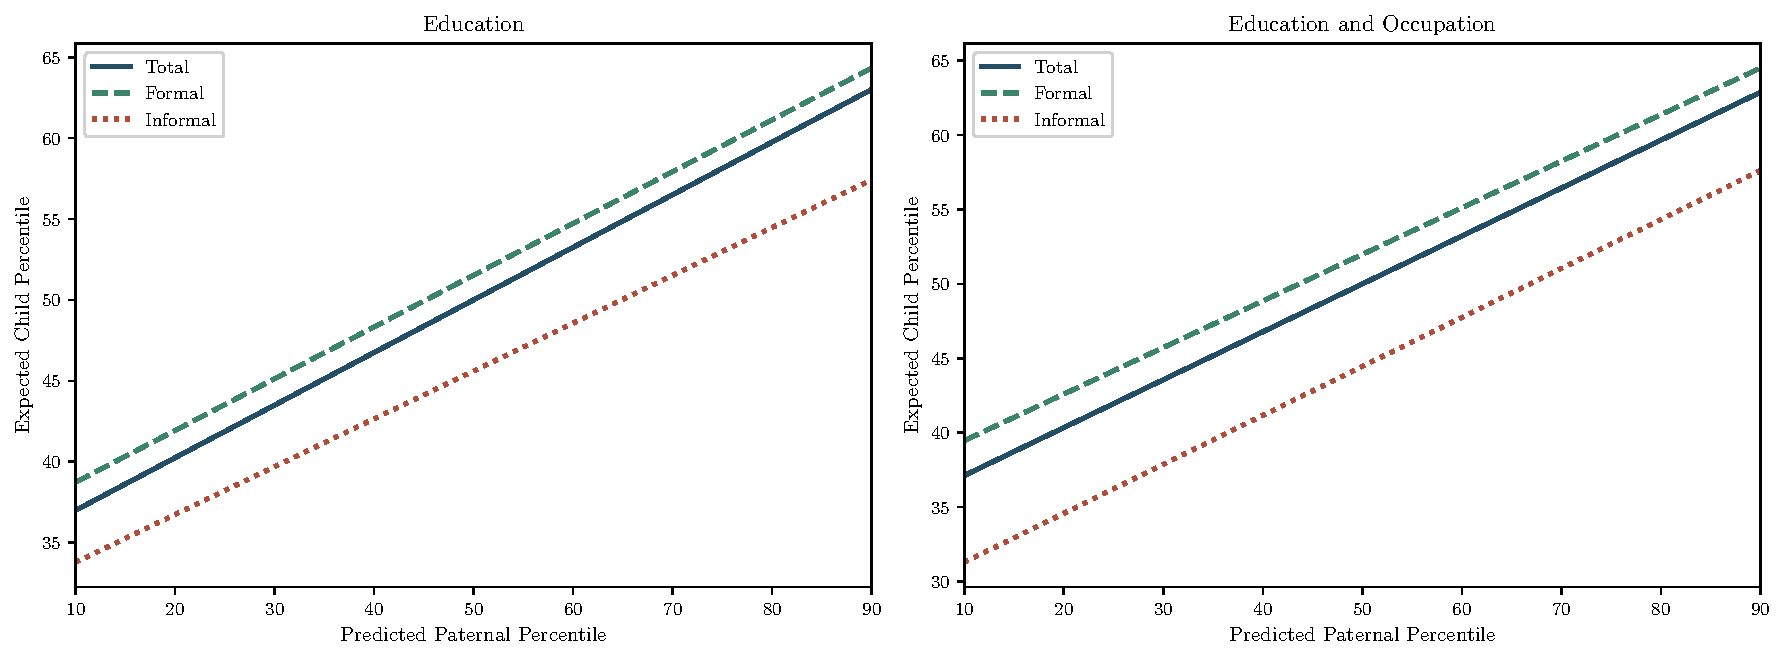
\includegraphics[width=0.95\textwidth]{../../figures/p1/rank_sector.pdf}
    \caption{Rank-rank fitted lines by sector (sons 25--40). Predicted paternal percentile vs.\ expected son percentile.}\label{fig:rank-sector}
\end{figure}

\subsection{Multiple Imputation of Paternal Income and Status}\label{sec:mi}
We restrict this extension to 6,498 sons aged 25--35 with known pension status. Paternal formality is proxied by historic affiliation ($o11 \in 1$--$6$ vs.\ $7$) while the son's is current contribution ($o29$); the two indicators differ in meaning. Log incomes follow a bivariate normal residual model with assumed correlation $\rho$:
\begin{equation}
    L_{pi} = \mu_{pi} + \varepsilon_{pi}, \quad L_{hi} = \mu_{hi} + \varepsilon_{hi}, \quad (\varepsilon_p,\varepsilon_h)^{\prime} \sim N_2(0,\Sigma_\rho).
    \label{eq:mi-model}
\end{equation}
Status follows a logistic model in predictors, age profile and log income. For each scenario $\rho \in \{0, 0.3, 0.6\}$ we generate $M=100$ versions: coefficients and variances are drawn from normal and inverse-chi-square posteriors, then paternal income and affiliation are imputed conditional on the son's observed residual.\footnote{See \texttt{source/mobility.py} (\texttt{multiple\_imputation}, seed 17102026) and \texttt{notebooks/07\_nunez\_miranda.ipynb}, Sec.~4. Same data-generating process as the reference implementation; the random engine differs so figures match within Monte Carlo error, not exactly.}

Within each imputation, paternal percentiles are recomputed over all 6,498 cases and rank-rank slopes are estimated for the four father-son combinations (F-F, F-I, I-F, I-I), then pooled with Rubin's rules.\footnote{Combined slope $\bar{\beta} = M^{-1}\sum \hat{\beta}^{(m)}$, total variance $T = \bar{U} + (1+M^{-1})B$ with Barnard-Rubin degrees of freedom.} Table~\ref{tab:mob-mi} shows the cotizante-son criterion: the affiliated-father/contributing-son slope is 0.168, 0.355 and 0.564 under $\rho = 0$, $0.3$ and $0.6$. The spread across scenarios reflects non-identified residual dependence, not something more imputations would resolve.

\begin{table}[H]
    \centering
    \caption{Multiple imputation: combined slopes by scenario (son = contributor)}\label{tab:mob-mi}
    \begin{tabular}{lcccc}
        \toprule
        $\rho$ & Father--son & Slope & 95\% interval & Mean $N$ \\
        \midrule
        0.0 & F-F & 0.168 & [0.130; 0.206] & 3,677 \\
        0.0 & F-I & 0.220 & [0.128; 0.311] & 971 \\
        0.0 & I-F & 0.116 & [0.045; 0.186] & 1,268 \\
        0.0 & I-I & 0.131 & [0.007; 0.256] & 582 \\
        0.3 & F-F & 0.355 & [0.319; 0.390] & 3,683 \\
        0.3 & F-I & 0.492 & [0.411; 0.572] & 966 \\
        0.3 & I-F & 0.294 & [0.229; 0.360] & 1,262 \\
        0.3 & I-I & 0.431 & [0.323; 0.538] & 587 \\
        0.6 & F-F & 0.564 & [0.535; 0.593] & 3,688 \\
        0.6 & F-I & 0.726 & [0.667; 0.785] & 960 \\
        0.6 & I-F & 0.490 & [0.430; 0.549] & 1,257 \\
        0.6 & I-I & 0.675 & [0.598; 0.753] & 593 \\
        \bottomrule
    \end{tabular}
    \vspace{0.2em}
    \flushleft\footnotesize{\textit{Note:} 100 imputations per scenario; F = affiliated father / contributing son. Intervals use Barnard-Rubin degrees of freedom.}
\end{table}

Figure~\ref{fig:mi-sens} shows the sensitivity: slopes rise with $\rho$ in all four groups, and the ordering F-F $<$ F-I is descriptive, not a tested difference. Conditioning on income-related states selects different distributions, so a higher slope means stronger relative association within the group, not a better outcome or upward mobility.

\begin{figure}[H]
    \centering
    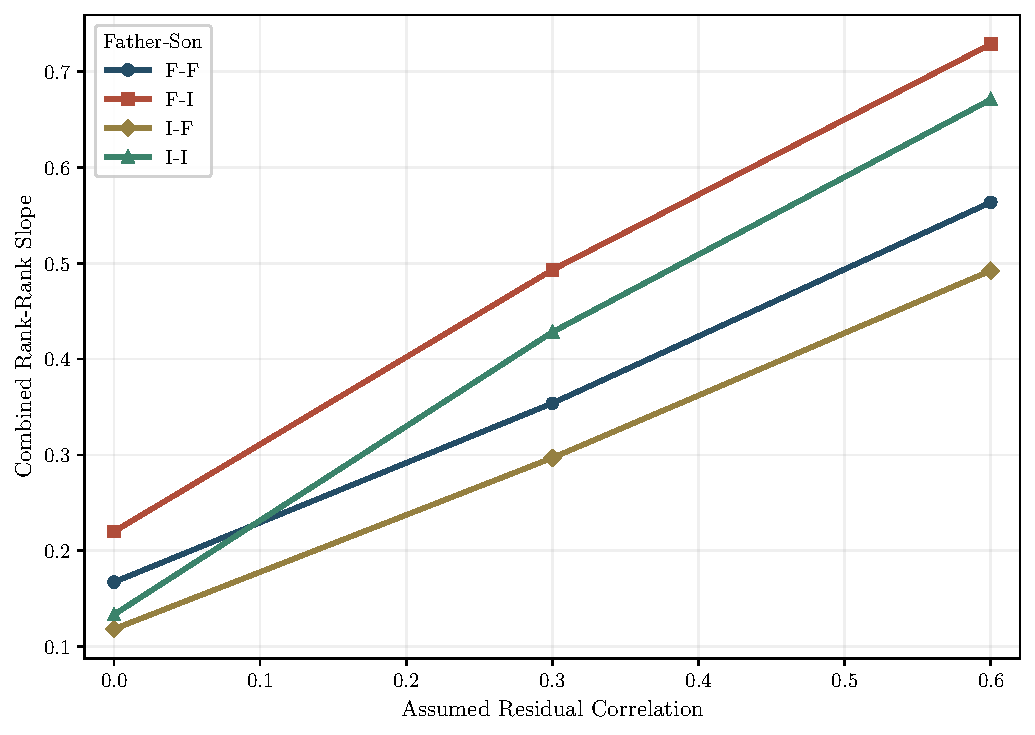
\includegraphics[width=0.70\textwidth]{../../figures/p1/sensibilidad_MI.pdf}
    \caption{Sensitivity of combined slopes to the assumed residual correlation. F = affiliated father / contributing son.}\label{fig:mi-sens}
\end{figure}
